% !Mode:: "TeX:UTF-8"
%% 请使用 XeLaTeX 编译本文.
% \documentclass{WHUBachelor}% 选项 forprint: 交付打印时添加, 避免彩色链接字迹打印偏淡. 即使用下一行:
 \documentclass[forprint]{WHUBachelor}
\usepackage{listings}
\usepackage{xcolor}

\lstset{
	language=python,  %代码语言使用的是matlab
	frame=shadowbox, %把代码用带有阴影的框圈起来
	rulesepcolor=\color{red!20!green!20!blue!20},%代码块边框为淡青色
	keywordstyle=\color{blue!90}\bfseries, %代码关键字的颜色为蓝色,粗体
	commentstyle=\color{red!10!green!70}\textit,    % 设置代码注释的颜色
	showstringspaces=false,%不显示代码字符串中间的空格标记
	numbers=left, % 显示行号
	numberstyle=\tiny,    % 行号字体
	stringstyle=\ttfamily, % 代码字符串的特殊格式
	breaklines=true, %对过长的代码自动换行
	extendedchars=false,  %解决代码跨页时,章节标题,页眉等汉字不显示的问题
	%   escapebegin=\begin{CJK*},escapeend=\end{CJK*},      % 代码中出现中文必须加上,否则报错
	texcl=true}

\begin{document}
%%%%%%% 下面的内容, 据实填空.

\miji{ }                                      % 密级. 没有就空着.
\StudentNumber{202010311229} % 填写自己的学号

\title{操作系统课程设计\\网络聊天室}
\Etitle{Operation System Course Design} % 英文题目
\author{孙思进}                            % 作者名字
\Eauthor{Sijin Sun}            %作者英文名
\Csupervisor{毕坤\quad 老师}        %指导教师中文名、职称
\Esupervisor{Teacher Kun Bi}     %指导教师英文名、职称
\Cmajor{计算机科学与技术}                  % 专业中文名
\Emajor{Computer Science and Technology}% 专业英文名
\Cschoolname{信息工程学院}          % 学院名
\Eschoolname{College of Information Engineering} %学院英文名. 不确定的话, 请看一下自己学院的网页上是怎么写的. 别搞错了!
\date{二〇二一年十一月}                    % 日期, 要注意和英文日期一致!!
\Edate{October, 2021}                       % 英文封面日期

%-----------------------------------------------------------------------------
\pdfbookmark[0]{封面}{title}         % 封面页加到 pdf 书签
\maketitle
\frontmatter
\pagenumbering{Roman}              % 正文之前的页码用大写罗马字母编号.
%-----------------------------------------------------------------------------
% !Mode:: "TeX:UTF-8"
\thispagestyle{empty}
\renewcommand{\baselinestretch}{1.5}  %下文的行距

\begin{cnabstract}
本报告介绍了操作系统课程设计作品:《网络聊天室》的原理组成。本软件通过$Pythony$语言编写,
使用$ Socket $通信的方式,实现了点对点、点对面的文本信息传递功能,巧妙利用$ FTP $服务器的功能实现了图片
传输、视频传输、音频传输等功能。最终的成品运行在阿里云主机上,实现真正意义上的网络聊天功能。



\end{cnabstract}
\par
\vspace*{2em}

\cnkeywords{操作系统; 网络聊天室; $ socket $; $ C\&S $ }
\\
\enkeywords{Operation System;Internet Chat; socket;C\&S}
    % 加入摘要, 申明.
%==========================把目录加入到书签==============================%%%%%%
\pdfbookmark[0]{目录}{toc}
\tableofcontents
\mainmatter %% 以下是正文
%%%%%%%%%%%%%%%%%%%%%%%%%%%--------main matter-------%%%%%%%%%%%%%%%%%%%%%%%%%%%%%%%%%%%%
\chapter{引言}
\section{背景}
二零二一年正是$ 5G $通信的商用元年,回顾初代互联网的诞生,通信方式改善了人们的生活,从最初的短信单向通信,到$ Microsoft \; MSN$ ,从$ Xiaomi \;$ 米聊,到 $Tencent \; QQ $,再到$Tencent \; WeChat$,大大提高了人们的沟通方式。
\begin{figure}[ht]
	\centering
	
\includegraphics{msn.jpg}
	\caption{$MSN \;$中国}
	\label{fig:1}
\end{figure}

\begin{figure}[ht]
	\centering
	
\includegraphics{qq.jpg}
	\caption{$Tencent \; QQ $}
	\label{fig:2}
\end{figure}

\begin{figure}[ht]
	\centering
	
\includegraphics{wechat.jpg}
	\caption{$Tencent \; WeChat $}
	\label{fig:3}
\end{figure}
\section{编程语言}

本软件主要采用$Python \; 3.7$进行编写,使用的库如表\ref{table:1}所示
\begin{table}[ht]\centering
	\caption{$Python$配置包}
	\label{table:1}
	\begin{tabular}{ccl}
		\hline
		序号 & 名称       & 功能                           \\ \hline
		1  & $Socket$    & 实现点对点通信                   \\
		2  & $Tkinter$   & 图形化$GUI$                      \\
		3  & $openCV$    & 显示图片、视频、音频等多媒体信息    \\
		4  & $ftplib$    & 传输文件                           \\
		5  & $json$      & 打包数据,生成嵌套字                \\
		6  & $threading$ & 实现多线程                          \\
		7  & $py2neo$    & $Neo4j$在$Python \;$运行的基础库     \\ \hline
	\end{tabular}
\end{table}

\section{配置环境}

本软件的编译和运行均基于表\ref{table:2}的环境下配置,此外,设计报告撰写使用\LaTeX{}。

\begin{table}[ht]\centering
	\caption{系统环境}
	\label{table:2}
	\begin{tabular}{ccl}
		\hline
		序号 & 名称        & 版本                                                        \\ \hline
		1  & 客户端       & $Windows \;10 \; Professior$                              \\
		2  & 服务器端      & $Windows \; 10 \; DataBase $\\
		3  & $PyCharm$ & $PyCharm \; Community \; 2021.2.2$                        \\
		4  & $Java$    & $Java \; JDK \; 18$                                       \\
		5  & \LaTeX{}   & $TexLive \; 2020$                                      \\
		6  & $Neo4j$   & $Neo4j \; Community 4.3.5$                                \\ \hline
	\end{tabular}
\end{table}

\chapter{设计分析}
\section{性能分析}

编写一个网络聊天室,对于服务器来说,需要做到如下几个功能:

\begin{itemize}
	\item 直接
	\item 快速
	\item 低延迟
	\item 安装便捷
	\item 多媒体化
\end{itemize}

涉及到点对点通信,$socket$的通信方式显然是首要选择方式,它基于$TCP/IP$协议,实现了点对点的通信,并且传输速度不受其他因素限制。由于采用嵌套字传输方式,在安全方面可能存在一定风险,有被抓包分析的可能性。

对于私人和多人聊天有着不同的功能要求,私人聊天之间需要较高的加密程度,确保信息安全;而多人公开聊天中,则需要考虑多并发的情况,对于一个消息文本,短时间瞬发需求极大,软件需要保证不漏发、不错发的前提下高效率的传输信息。

本软件使用python语言开发,不涉及库文件的安装情况下,源文件不到1mb,并且python的同一个代码源文件可以同时在$Linux \; MacOS \; Windows$系统运行,实现了轻量化的设计需求。

在高带宽的信息化时代下,软件不能仅仅局限于文本的收发,消息的种类更应该多样化,复杂化。因此,不仅要考虑文本的传输,更应该关注到图片、视频、语言的收发功能。

\section{需求分析}

为了做到高效的通信,减少用户端设备的硬件要求,本软件采用$ C/S $端的假设方式,$ C $端即为$ Client $:客户端,$ S $端即为$ Serve $:服务器端。

本软件初代运行在局域网中,将服务器端假设在局域网的某台电脑中,实现了群聊和单聊的通信功能。考虑到在一定程度上无法每时每刻连接内网的网关,故后续将本软件的服务器端架设在阿里云上,实现了广域网通信。

\begin{figure}[ht]
	\centering
	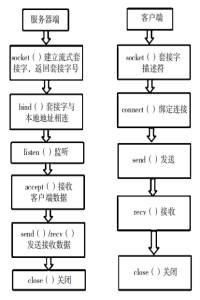
\includegraphics{tongxin.jpg}
	\caption{通信原理\upcite{r1}}
	\label{fig:5}
\end{figure}

客户端/服务器模型最终归结为一个“请求/应答”的关系。一个请求总是第一个颁发给客户端,然后服务器总是被动地接收请求,返回结果给客户需要。在客户端发送一个请求时,服务过程一直处于休眠状态。在一个客户端请求时,服务过程是“唤醒”和为客户提供服务,根据客户的要求进行回复。\upcite{r2}因此采用socket框架。
\section{功能分析}

如图\ref{fig:6}所示,整个软件的功能主要分为几个方面:

\begin{figure}[ht]
	\centering
	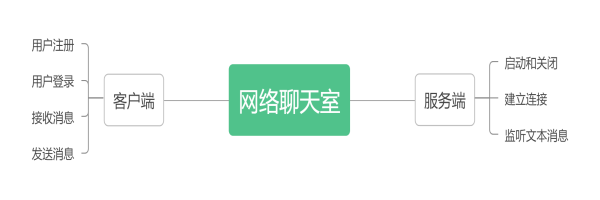
\includegraphics{chat1.png}
	\caption{网络聊天室需求分析}
	\label{fig:6}
\end{figure}

对于客户端而言,主要负责用户的登录和注册,以及最重要的收发消息。

对于服务器端而言,负责处理收到的文本,将其转发到各个用户所在的$ip$地址的端口上。
\section{数据库}

数据库使用了$ Neo4j $,一种基于离散数学中图论原理的轻量数据库,普遍被称为知识图谱,相比较传统的$MySql$、$SqlLite$而言,其基本的结构由节点($Node$)、关系($Relationship$)
和标签($Label$)组成,通过这三个属性可以构建出传统数据库没有的功能。

如图所示,源文件为一个有关于心理测试的调查信息,通过简单的$NLP$处理后,可以将原来的字段拆分成多个关系,形成有向关系网路。

\begin{figure}[ht]
	\centering
	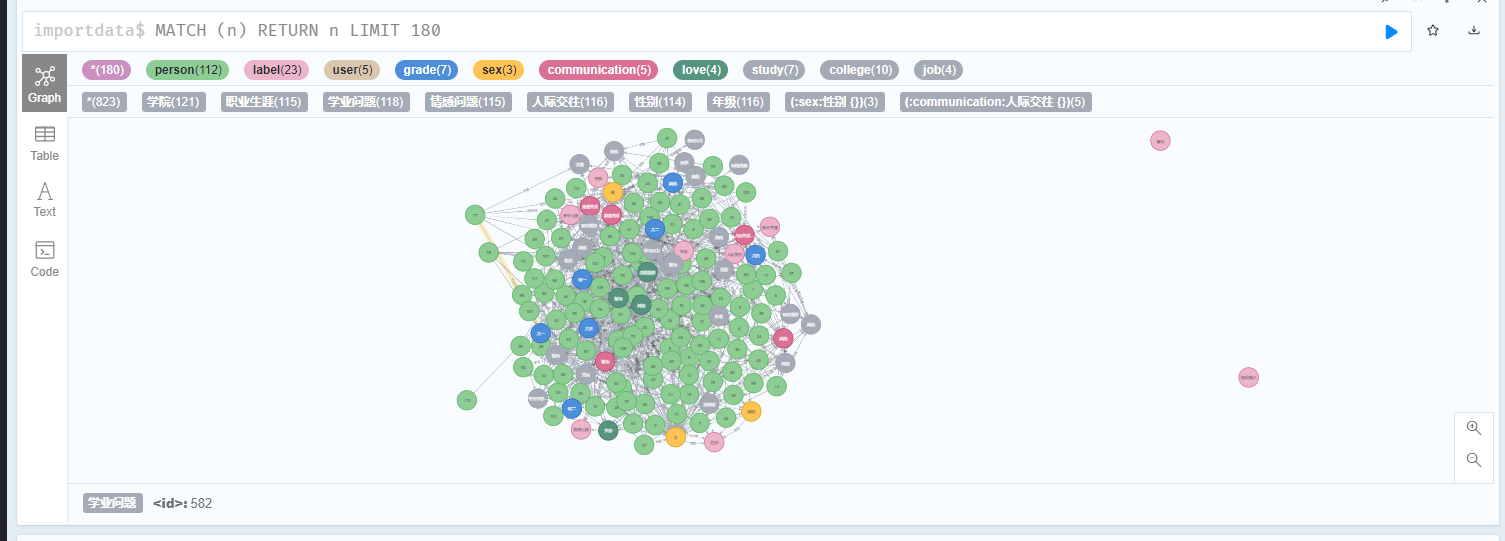
\includegraphics[width=\textwidth]{neo4j.png}
	\caption{通过$ Neo4j $形成的复杂关系图}
	\label{fig:7}
\end{figure}
调用$Neo4j$数据库的查询极为便捷,其编写语言全部源于$ Java (jdk-12)$,不仅支持在$Java$中查询,更能在
$ Python $、$C++$等主流语言中调用,同时也可以以$jpg$、$png$和$json$等多种格式保存。

此外,$Neo4j$可以储存的数据极为庞大,如\ref{table:2}所示,对于一个网络聊天室来说足矣。

\begin{table}[ht]\centering
	\caption{$Neo4j$数据容纳量}
	\label{table:3}
	\begin{tabular}{ccc}
		\hline
		S.No & 构建基块 & 数量      \\ \hline
		1    & 节  点 & 约 350 亿 \\
		2    & 关  系 & 约 350 亿 \\
		3    & 标  签 & 约 275 亿 \\ \hline
		
	\end{tabular}
\end{table}

\chapter{系统功能实现}

\section{登录}
\subsection{原理}
登录部分涉及到验证、确认等操作,流程如图\ref{fig:8}所示:

\begin{figure}[ht]
	\centering
	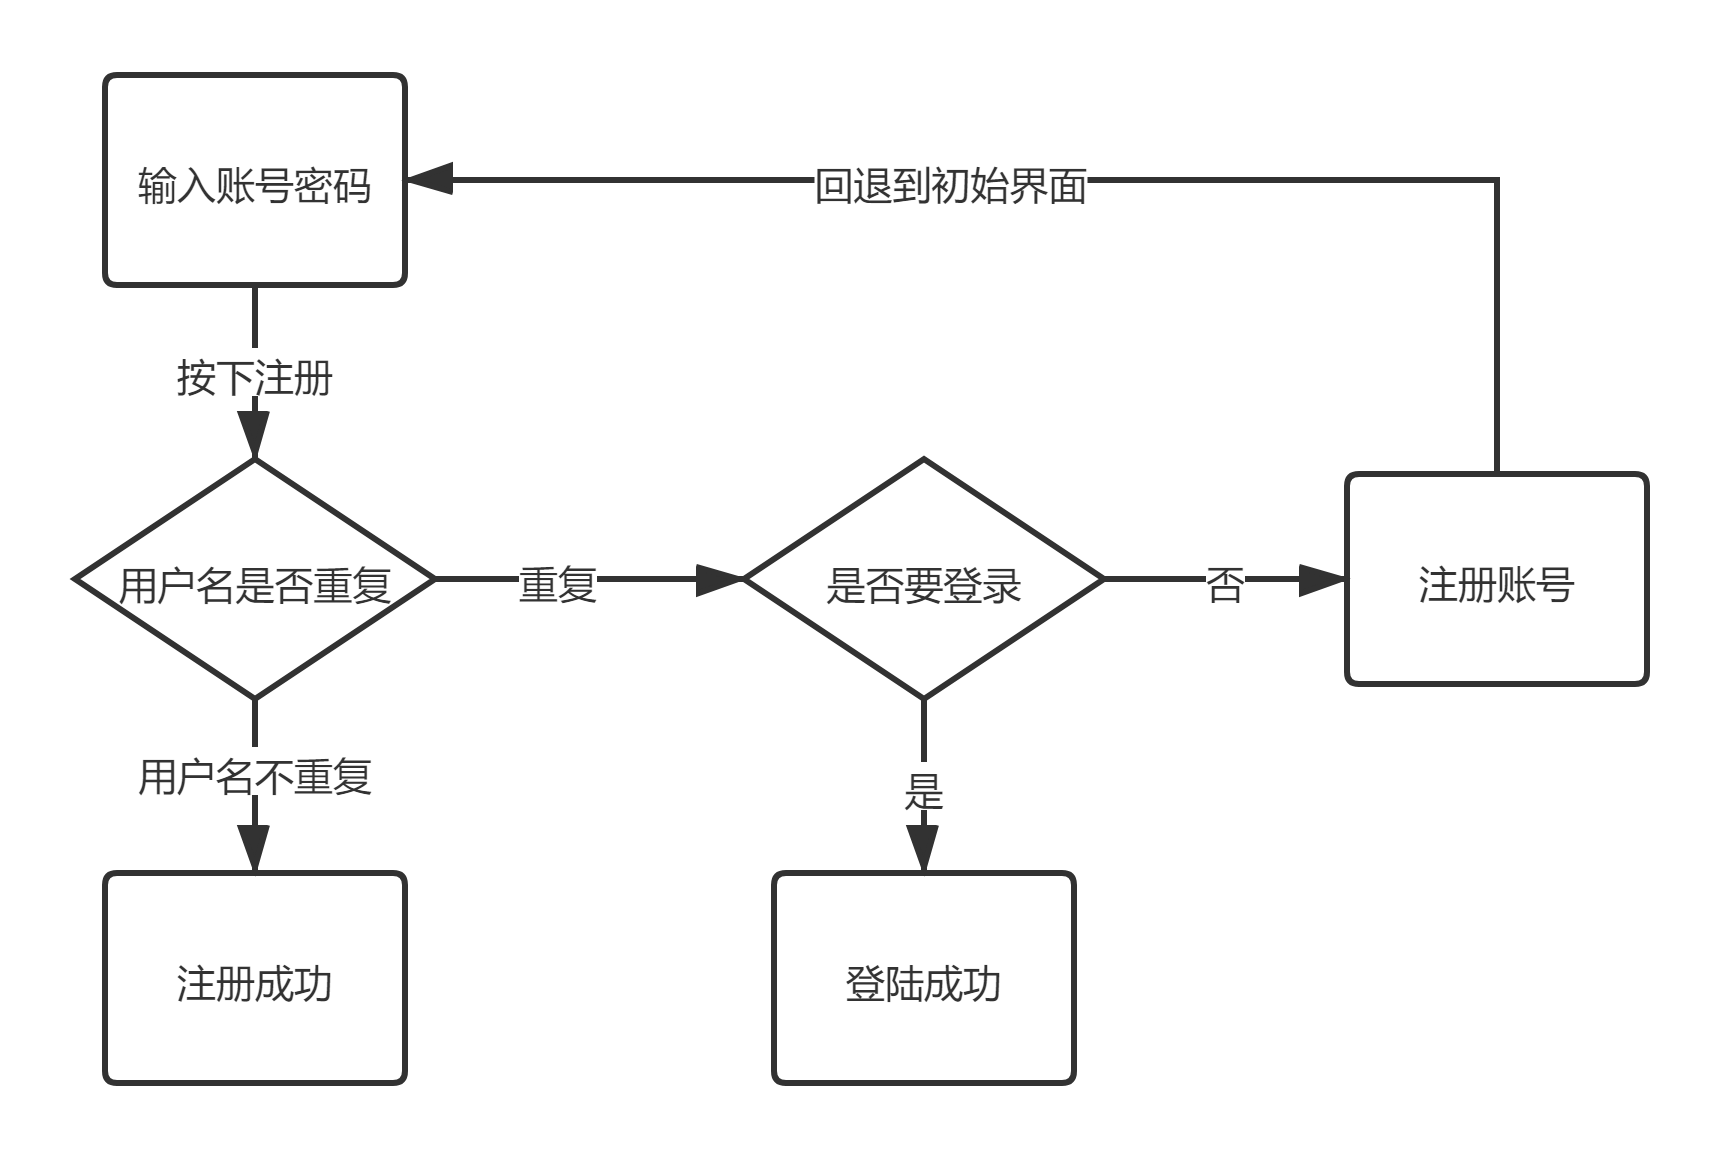
\includegraphics[width=\textwidth]{login.png}
	\caption{登录系统流程图}
	\label{fig:8}
\end{figure}

\subsection{功能设计}

用户在输入账号和密码以后,按下$Enter$或者登录按钮,程序将输入的字符串转化为嵌套字,传输到服务器端,服务器端启动数据库查询功能,如果用户名存在,但是密码错误,
返回-1,客户端弹出“密码错误”提示;如果用户名不存在,返回0,客户端弹出“用户名不存在”提示;如果用户名和密码都匹配,返回1,客户端弹出“登录成功”提示,跳转到聊天框。包括注册系统在内的返回值均列在了表\ref{table:3}中。
\begin{table}[]
		\caption{登录\&注册 返回值}
	\label{table:3}
	\begin{tabular}{ccl}
		\hline
		返回值 & 提示     & 备注                         \\ \hline
		-1  & 密码错误   & 用户输入了存在的账号,但是密码不匹配,保留该界面   \\
		0   & 用户名不存在 & 用户输入了不存在的账号,不进行密码匹配,保留该界面  \\
		1   & 登录成功   & 用户输入了匹配的账号和密码,登陆成功,跳转到聊天栏  \\
		2   & 用户名已存在 & 用户注册的账号已经存在,保留注册界面         \\
		3   & 注册成功   & 用户注册账号成功,保留注册界面录 \\ \hline
	\end{tabular}
\end{table}

\section{注册}
\subsection{原理}
使用流程图\ref{fig:9}简要的画出了注册系统的设计思路。
\begin{figure}[ht]
	\centering
	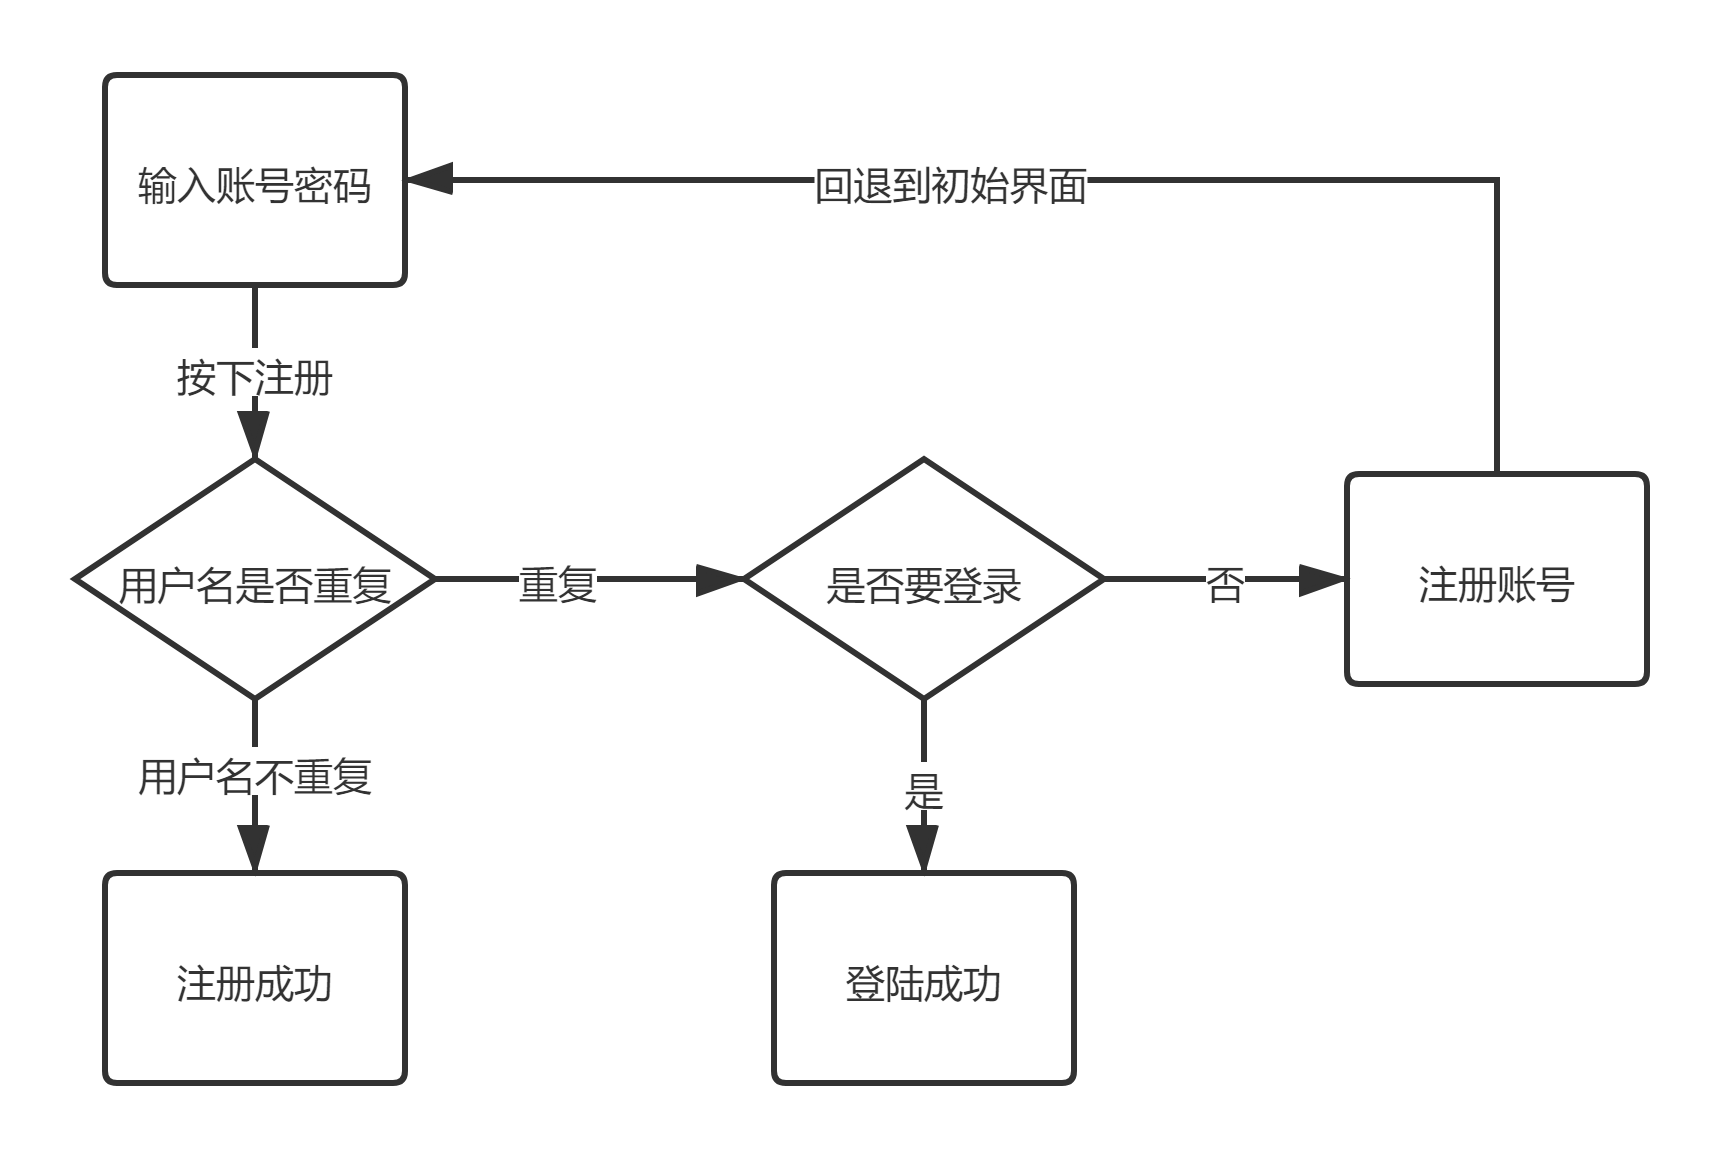
\includegraphics[width=\textwidth]{regi.png}
	\caption{注册系统流程图}
	\label{fig:9}
\end{figure}

\subsection{功能设计}

用户在输入账号和密码以后,按下注册按钮,和登录相同,服务器先匹配用户名是否存在,如果存在,返回2,客户端提示“用户名已存在”;否则,返回3,客户端提示”注册成功“,此时,按下登录即可使用注册的账号进行登录,返回值对于的效果见表\ref{table:3}所示。

\section{文本发送}
\subsection{原理}
通过流程图\ref{fig:10}展示了文本发送的编写方法。
\begin{figure}[ht]
	\centering
	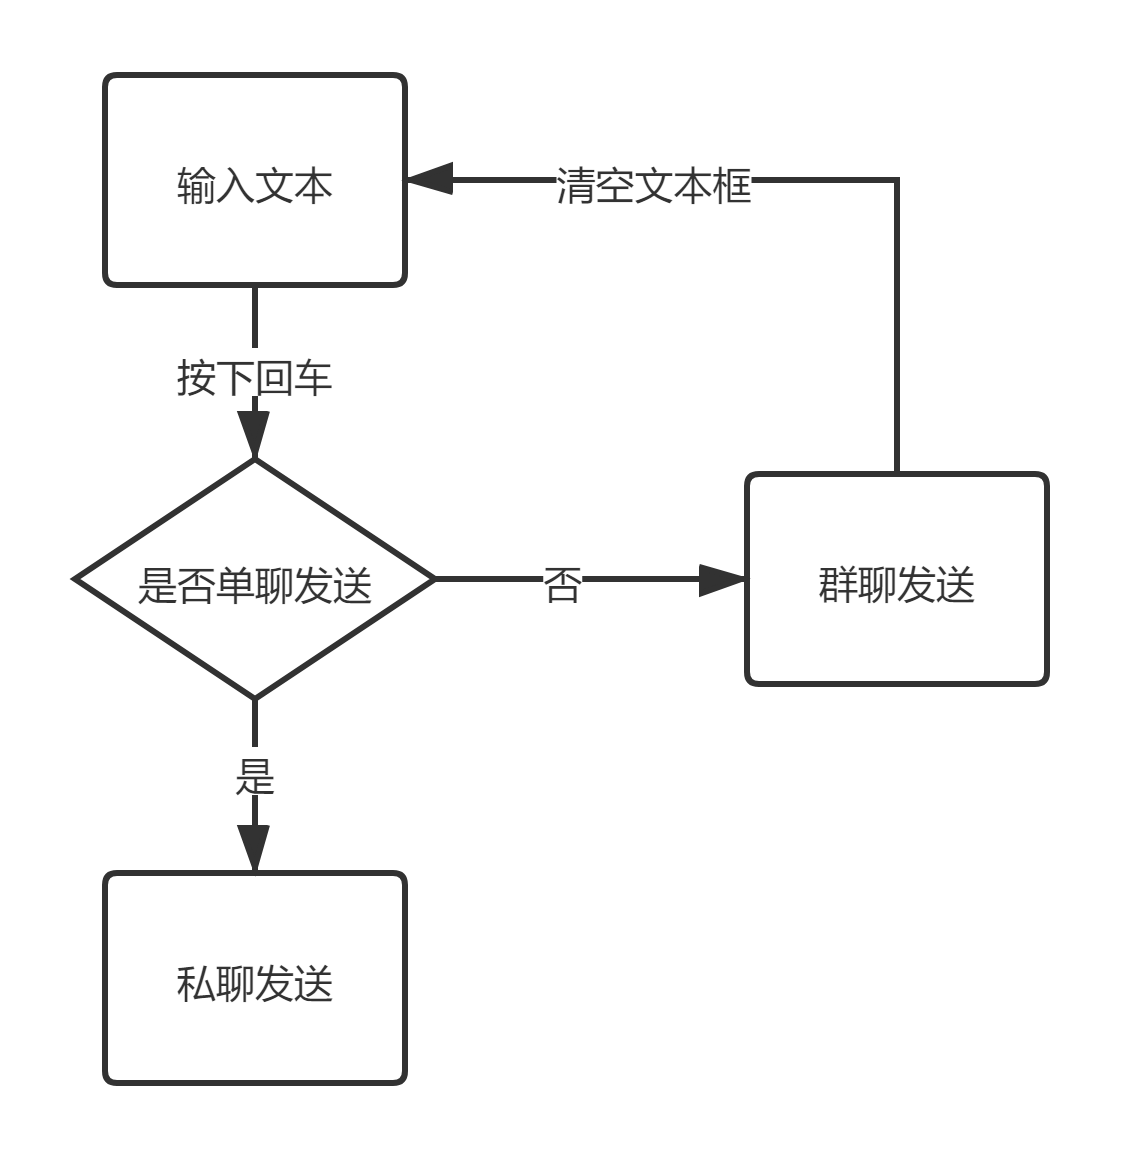
\includegraphics[width=\textwidth]{text.png}
	\caption{文本发送流程图}
	\label{fig:10}
\end{figure}

\subsection{功能设计}

当登录成功后,将显示聊天窗口,左上角部分为文本显示区域,显示别人发送的群聊、单聊文本;左下角为输入框,输入文本,其右边是发送按键,按下后即可发送;右侧是功能栏,包含发送图片、发送视频等功能。

若用户想要群聊,只需要输入文本$Text_0$,每个人都会接收到文本$Text_0$;若用户想要单聊,则在原先需要输入的 $Text_0$ 后额外输入 $ \sim $  用户名,即字符串\ref{equ:3}:
\begin{equation}
	\label{equ:3}
	Text = Text_0 + \sim + UserName
\end{equation} 

例如,“我”想要和用户“Tom”私聊,对话内容是“你今天吃饭了吗?”,那么“我”应该输入字符串\ref{equ:4}。

\begin{equation}
	\label{equ:4}
	Text = \mbox{你今天吃了吗} \sim Tom
\end{equation} 


\section{图片}
\subsection{原理}
图片发送的实现运用了$FTP$服务器,间接实现了图片的传输,同时也能实现聊天记录保存的功能。如流程图\ref{fig:11}所示,图片传输的方式:

\begin{figure}[ht!]
	\centering
	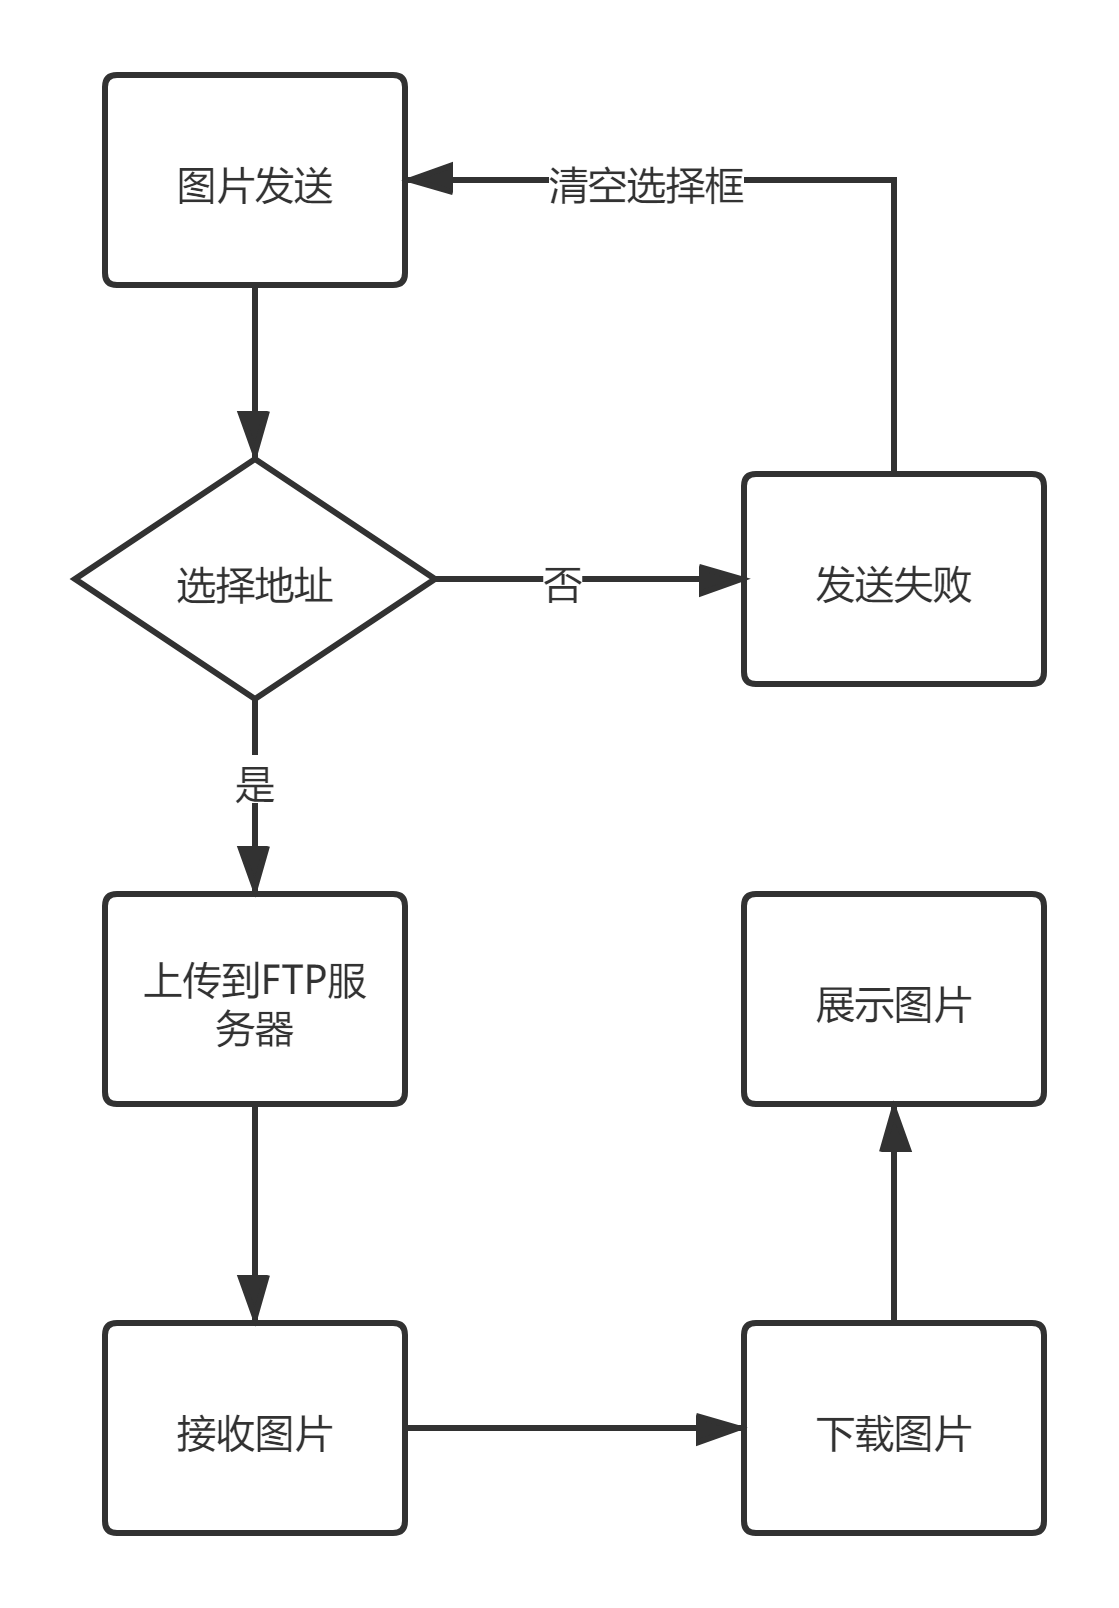
\includegraphics[width=0.3\textwidth]{picsend.png}
	\caption{图片发送流程图}
	\label{fig:11}
\end{figure}
\subsection{功能设计}

首先使用$openCV$的$imread$功能读取图片,转化为点矩阵,再使用$FtpLib$模块连接$FTP$服务器,输入上传指令$STOR FileName$上传,输入$RETR$下载,再使用$imshow$函数显示图像,至此,完成了图片的传输和显示功能。

由于图片的读取和保存都使用$openCV$模块,这样可以确保图片的读写方式相同,避免出现$RGB565$和$RBG565$不同读取方式,提升了程序的鲁棒性。

\section{多媒体影像}
\subsection{原理}
多媒体文件发送的方式和图片发送相类似,也采用了$FTP$的间接方法,通过调用$openCV$模块实现视频、音频的播放。
\subsection{功能设计}

$openCV$提供了视频文件的读取方式$VideoCapture(FilePath)$,通过切割读取的视频每一帧,这时候视频转化为了图片,可以沿用图片的读取方式来显示。

\section{队列}
\subsection{优先级}
当服务器处于高并发状态时,如何才能保证消息的正常收发呢?这时就需要使用队列了。

如图\ref{fig:12}所示,队列的工作原理遵循“先进先出”的原则,这样就可以保证先发送的消息先传输到各个用户,后发送的消息被后接受,从而确保时序的稳定。


\begin{figure}[ht]
	\centering
	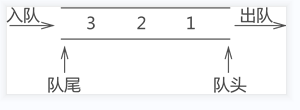
\includegraphics[width=0.5\textwidth]{duilie.png}
	\caption{队列优先}
	\label{fig:12}
\end{figure}
\subsection{应用}
在创建完队列后,如果有某个用户发送消息,那么这个消息将传入队列的最前端,记为$Q_0$,若第一个消息还未被处理,第二个消息又被传入,那么第一个消息的位置将转移到$Q_1$,第二个消息的位置代替原先第一个消息的位置,即$Q_0$。

\section{消息记录}

\subsection{存储}

消息的存储使用数据库$Neo4j$,通过建立节点存放消息,其标签分别为$sender$、$receiver$和$text$,使用$Py2neo$可以较为快速的创建一个节点,其语法如代码\ref{equ:5}。

\begin{equation}
	\label{equ:5}
	CreateRelationship(graph, label1, attrs1, label2, attrs2, name)
\end{equation}

\subsection{读取}
这时我们可以通过数据库查询代码\ref{equ:6}来获取某个发送者发送的消息,通过代码\ref{equ:7}来获取某个人接收到的消息。

\begin{equation}
	\label{equ:6}
	MATCH \; (n:sender) \; RETURN \; n:text \;
\end{equation}

\begin{equation}
		\label{equ:7}
	MATCH \; (n:receiver) \; RETURN \; n:text \;
\end{equation}

我们既可以通过$Neo4j$输入该命令,也可以在$Python$添加这个语段,输出以json格式打包,可以快读在其他的数据读取程序中运行。

\section{嵌套字}
无论使用哪一种地址家族,嵌套字的类型只有两种。一种是面向连接的套接字,即:在通信之前一定要建立一条连接,就像跟朋友打电话时那样,这种通信方式也被成为“虚电路” 或 “流套字节”。面向连接的通信方式提供了顺序的、可靠的、不会重复的数据传输,而且也不会被加上数据边界。这也意味着,每一个要发送的信息,可能会被拆分成多份,每一份都会不多不少地正确到达目的地。然后被重新安顺序拼装起来,传给正在等待的应用程序。

无论你使用哪一种地址家族,嵌套字的类型只有两种。一种是面向连接的套接字,即:在通信之前一定要建立一条连接,就像跟朋友打电话时那样,这种通信方式也被成为“虚电路” 或 “流套字节”。面向连接的通信方式提供了顺序的、可靠的、不会重复的数据传输,而且也不会被加上数据边界。这也意味着,每一个要发送的信息,可能会被拆分成多份,每一份都会不多不少地正确到达目的地。然后被重新安顺序拼装起来,传给正在等待的应用程序。
\section{云服务器}
\subsection{概述}
本软件运行在阿里云服务器,公网$IP$地址为\ref{equ:1},内网$IP$地址为\ref{equ:2}:
\begin{equation}
	\label{equ:1}
	47.100.93.63
\end{equation}
\begin{equation}
	\label{equ:2}
	172.24.12.68
\end{equation}

\subsection{端口开放}
阿里云平台涉及到$Neo4j$、$FTP$等多个服务器的同时部署,在表\ref{table:4}中列出了所有需要使用到的端口。

\begin{table}[ht]
	\caption{端口及其作用}
	\label{table:4}
	\begin{tabular}{ccl}
		\hline
		端口号 & 用途     & 备注                         \\ \hline
		21  & $FTP$服务器 - $Port$ 端口   & $FTP$源文件位于C:/FTP/   \\
		80   & 服务器首页端口   & $IIS$服务提供的主页  \\
		443   & 个人网页端口   & 个人博客主页的端口  \\
		1023-1033   & $FTP$服务器 - $Passive$& 为了确保连接稳定,开启$FTP$访问模式  \\
		6666   & 网络聊天室端口   & 提供聊天室对外的端口  \\
		7474   & $Neo4j$端口 & 知识图谱数据库的对外端口        \\
		8888   & $Jupyter \; Notebook$   & $Jupyter Notebook$的对外端口 \\ \hline
	\end{tabular}
\end{table}

\chapter{系统测试}
\section{登录界面}
登录界面如图\ref{fig:13}所示:

\begin{figure}[ht]
	\centering
	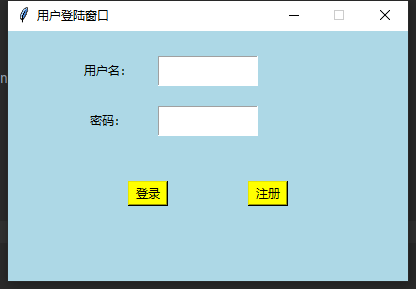
\includegraphics[width=0.3\textwidth]{loginui.png}
	\caption{登录UI}
	\label{fig:13}
\end{figure}

\subsection{按键提示}


\begin{figure}[htbp]
	\begin{minipage}[t]{0.5\linewidth}
		\centering
		\label{fig:14}
		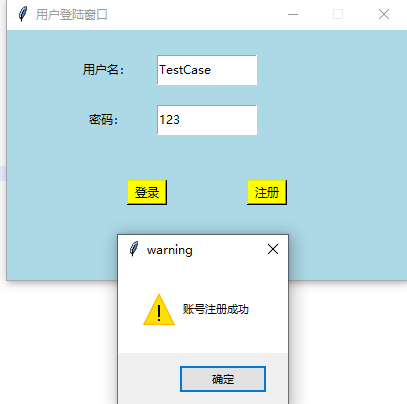
\includegraphics[height=4cm,width=4cm]{us.png}
		\caption{注册成功提示}
	\end{minipage}
	\begin{minipage}[t]{0.5\linewidth}
	\centering
	\label{fig:15}
	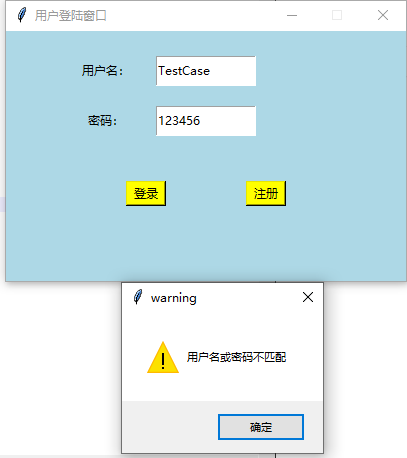
\includegraphics[height=4cm,width=4cm]{up.png}
	\caption{密码错误提示}
\end{minipage}
\end{figure}

上述图分别展示了注册成功和登录失败两种状态。


\begin{figure}[htbp]
	\begin{minipage}[t]{0.45\linewidth}
	\centering
	\label{fig:16}
	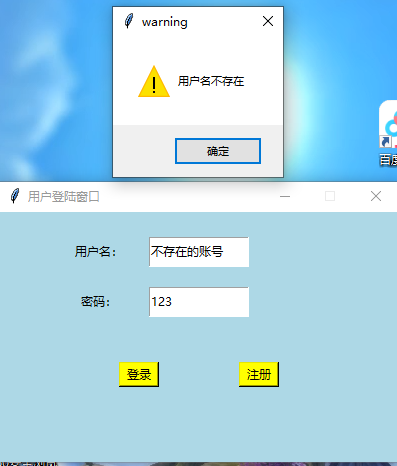
\includegraphics[height=3cm,width=3cm]{un.png}
	\caption{账号不存在提示}
	\end{minipage}%
	\begin{minipage}[t]{0.45\linewidth}
	\centering
	\label{fig:17}
	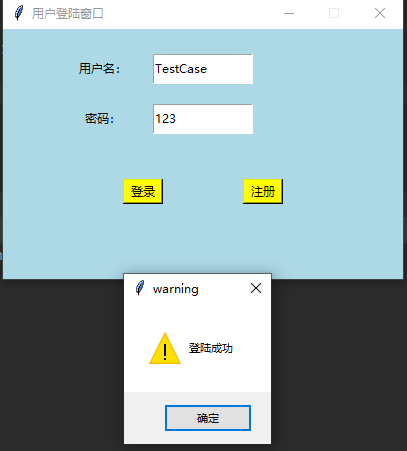
\includegraphics[height=3cm,width=3cm]{ls.png}
	\caption{登录成功}
\end{minipage}%
\end{figure}
上述图分别展示了登录成功和账号不存在两种状态。
\section{聊天界面}
聊天界面如图\ref{fig:18}所示:
\begin{figure}[ht]
	\centering
	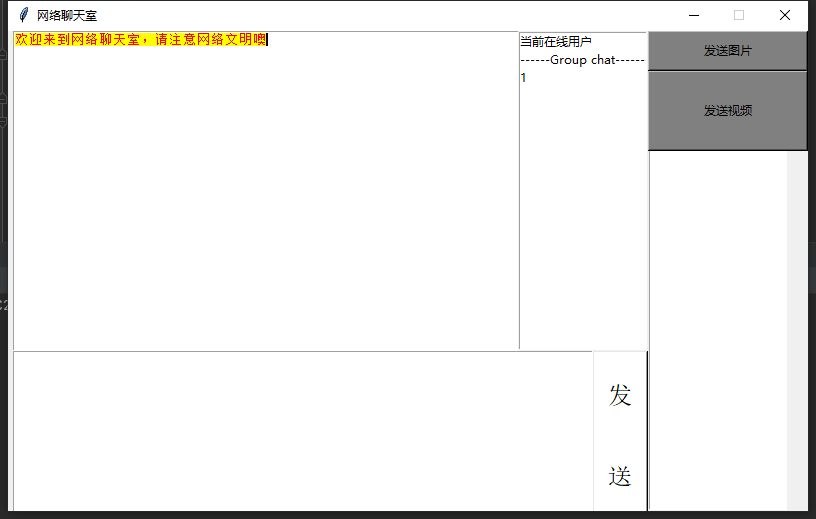
\includegraphics[width=1\textwidth]{chatui.png}
	\caption{聊天界面UI}
	\label{fig:18}
\end{figure}

当发送消息以后,如图\ref{fig:19}所示,信息框展示收到的信息。

\begin{figure}[ht]
	\centering
	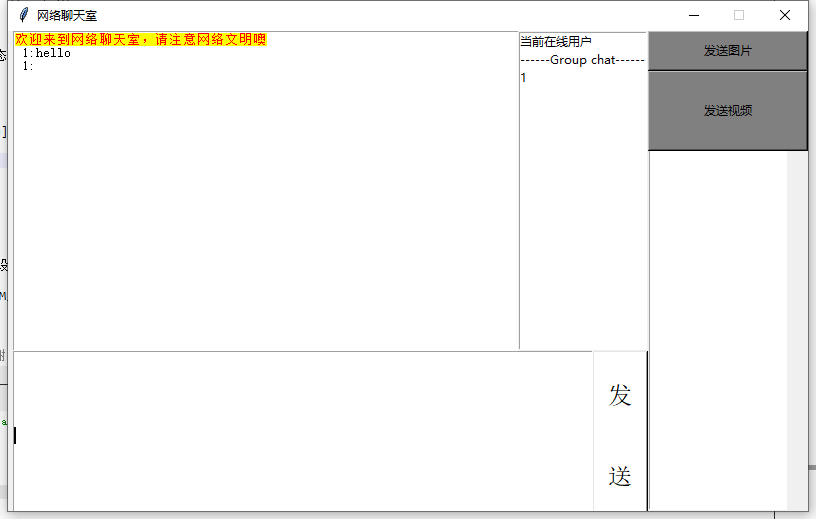
\includegraphics[width=0.60\textwidth]{send.png}
	\caption{聊天}
	\label{fig:19}
\end{figure}
\vspace*{2.5cm}
当发送图片以后,如图\ref{fig:20}所示,$openCV$打开图片。

当发送视频以后,如图\ref{fig:21}所示,$openCV$打开视频。

\begin{figure}[h]
	\begin{minipage}[t]{0.5\linewidth}
		\centering
		\label{fig:20}
		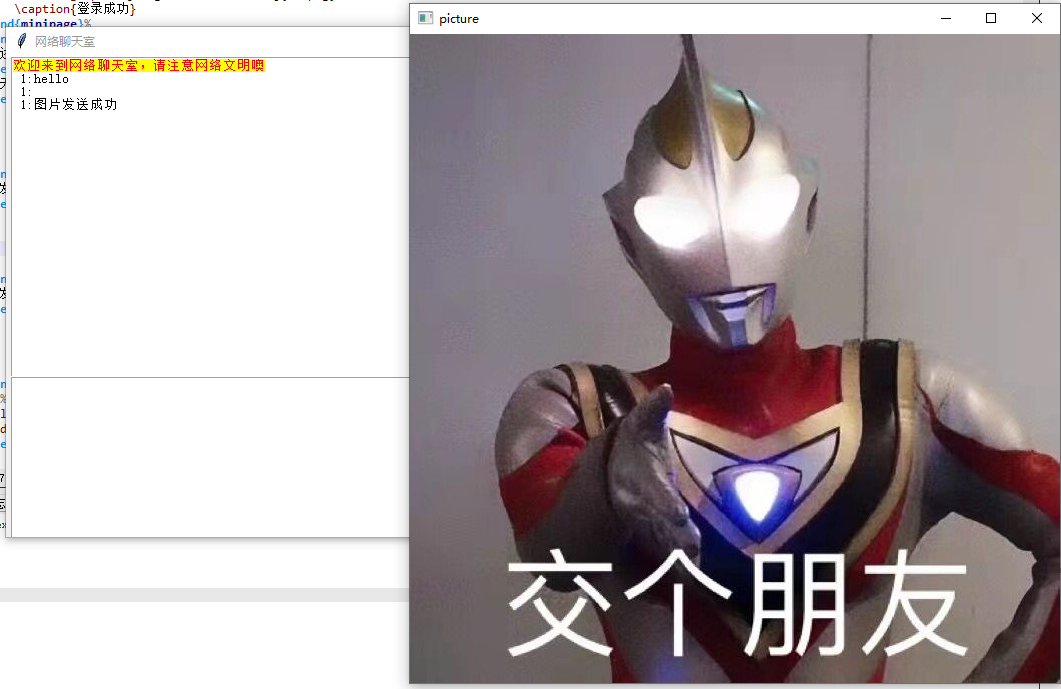
\includegraphics[height=3cm,width=3cm]{sendpic.png}
		\caption{发送图片}
	\end{minipage}%
	\begin{minipage}[t]{0.5\linewidth}
		\centering
		\label{fig:21}
		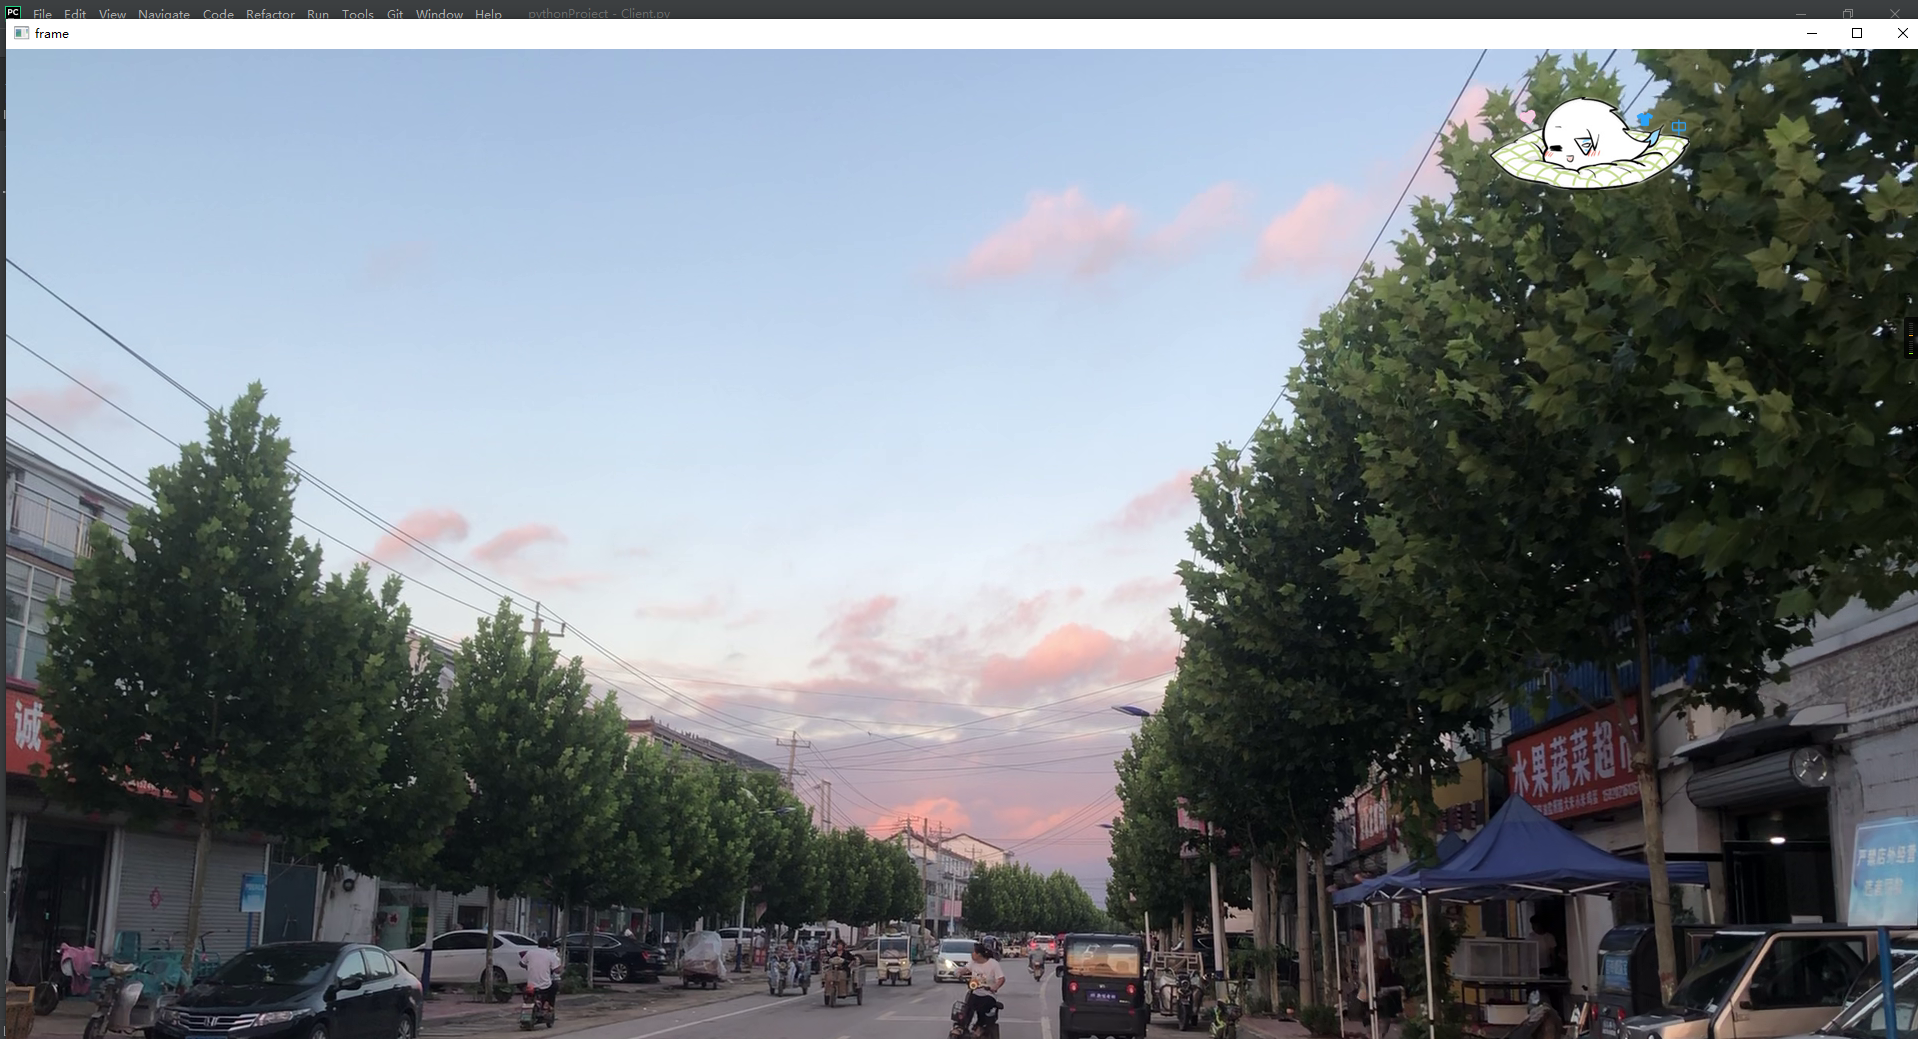
\includegraphics[height=3cm,width=3cm]{sendvid.png}
		\caption{发送视频}
	\end{minipage}%
\end{figure}
%%%=== 参考文献 ========%%%
\cleardoublepage\phantomsection
\addcontentsline{toc}{chapter}{参考文献}
\begin{thebibliography}{99}

  \bibitem{r1} 郭炳均,王思晗.网络聊天室的设计与实现[J].信息与电脑(理论版),2020,32(22):89-90.

  \bibitem{r2} 张淑坤.基于SOCKET嵌套字的IM系统设计与实现[J].数字技术与应用,2013(05):204.

\end{thebibliography}

%% !Mode:: "TeX:UTF-8"
%%%%%%%%%%%%%%%%%%%%%%%%%%%%-------致谢--------%%%%%%%%%%%%%%%%%%%%%%%%%%%%%%%%

\acknowledgement
\addcontentsline{toc}{chapter}{致谢}


感谢你, 感谢他和她, 感谢大家.











 %%%致谢

%%%-------------- 附录. 不需要可以删除.-----------
\appendix


\chapter{代码}

\section{客户端}

\begin{lstlisting}
	import os
	import socket
	import tkinter
	import tkinter.messagebox
	import threading
	import json
	import tkinter.filedialog
	from tkinter.scrolledtext import ScrolledText
	import demo.neo4j.Neo_Fun as NeoFun
	import cv2
	import numpy as np
	import ftplib
\end{lstlisting}

\section{客户端}
\begin{lstlisting}
	import os
	import socket
	import tkinter
	import tkinter.messagebox
	import threading
	import json
	import tkinter.filedialog
	from tkinter.scrolledtext import ScrolledText
	import demo.neo4j.Neo_Fun as NeoFun
	import cv2
	import numpy as np
	import ftplib
\end{lstlisting}
\end{document}



